%\documentclass[]{article}
\documentclass{scrartcl}
\usepackage{graphicx}
\usepackage[english]{babel}
\usepackage[a4paper]{geometry}
\usepackage{hyperref}
%opening
\title{Distributed Systems: Java RMI session 2/3}
\author{Jago Gyselinck, Armin Halilovic}

\begin{document}
	\maketitle

	\section{Overview}
	First, describe in 1 or 2 paragraphs the overview of your design. Which are the core
    parts/components and their responsibilities? This is not a sequential story! Next, at least the
    following design decisions should be discussed. \\


    \subsection{Serializable classes}
    The following classes are serializable: 
    \begin{itemize}
    	% CarRentalCompany is enkel remote, niet serializable :) 
		\item \texttt{Car, CarType, Quote, Reservation, ReservationConstraints}
		\item We made these classes serializable as data of their type has to be
		communicated between different distributed components. 
		\item An example of this could be the \texttt{getAvailableCarTypes} method which returns \texttt{Set<CarType>} and is made available in the \texttt{CarRentalCompanyRemote} interface. 
		The class \texttt{ReservationSession} makes use of this method, but resides on a different distributed component. For the method invocation on a remote reference of type \texttt{CarRentalCompanyRemote} to succeed, \texttt{CarType} must be serializable.
	\end{itemize}


    \subsection{Remote classes}
	The following classes are remotely accessible:
	\begin{itemize}
		\item \texttt{CarRentalCompanyRemote, RentalAgencyRemote,\\ ManagerSessionRemote, ReservationSessionRemote}
		\item We made these objects remotely accessible because their
		methods will be invoked from a non-local context, and remote references
		of their type will be passed along between different distributed components.
	\end{itemize}
	\newpage
	\subsection{Remote Object Locations}
    Which remote objects are located at the same host (or not) and why? \\
	\begin{itemize}
		\item Only the sessions (Manager and Reservation) and the Rental Agency
		reside on the same host. This allows the client to request a remote reference
		for the \texttt{CarRentalAgency} via the rmiregistry, and remote references to sessions can be requested via that remote reference. Those session remote references are kept in the remote \texttt{CarRentalAgency} object so they can be removed later. This organisation also has the advantage that when a method is invoked on a \texttt{(Manager/Reservation)Session} through a remote reference, the \texttt{CarRentalAgency} it has to interact with is a static object on the same component, so no remote interaction is required, and synchronization is easily achieved.
		\item All other remote objects are located on different hosts. The car rental companies reside on their own server each   
	\end{itemize}

	\subsection{Registering of remote objects}
    Which remote objects are registered via the built-in RMI registry (or not) and why? \\
%   allemaal toch?

    \subsection{Life cycle management}

    Briefly explain the approach you applied to achieve life cycle management of sessions. \\
%   getSession/removeSession

    \subsection{Synchronization}

    At which places is synchronization necessary to achieve thread-safety?
    Will those places become a bottleneck by applying synchronization?
%   overal waar meerdere calls een resource tegelijk kunnen aanpassen. dit maakt dan wel een bottleneck

	\section{Full class diagram}
    See 'class-diagram.jpg'.

	\section{Deployment diagram}
    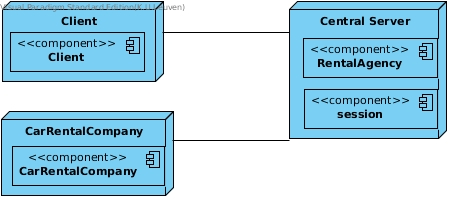
\includegraphics{deployment-diagram.jpg}

    \section{Sequence diagram}
    Sequence diagrams of the booking process have been included in the project.
    See 'sequence-diagram-success.jpg' and 'sequence-diagram-fail.jpg'.

    %    step  | client                     | agency                | crc
    %    1     | getNewReservationSession   | getRentalSession
    %    2.a   | checkForAvailableCarTypes  |                       | getAvailableCarTypes
    %    2.b   | addQuoteToSession(region1)
    %    2.c   | checkForAvailableCarTypes  |                       | getAvailableCarTypes
    %    2.d   | addQuoteToSession(region2)
    %    3     | confirmQuotes
    %    3.a.a |                            | confirmQuotes         | confirmQuote
    %    3.a.b |                            | confirmQuotes         | confirmQuote
    %    4.a   | clearSessions              | removeReservationSession
    %    3.b   |                            | confirmQuotes         | confirmQuote
    %    3.b.a |                            | confirmQuotes         | confirmQuote => ERROR
    %    3.b.c |                            | confirmQuotes         | cancelReservation
    %    4.b.a | throw ReservationException

\end{document}